\section{Software architecture views}
	This section discusses the system's architecture. The first subsection explains the high level architecture, such as the packages used and how to make parallel development possible. The program is composed of subsystems which depend on one another, this will be explained in the second subsection. The third subsection focuses on the relation between the hard- and software. Finally, the fourth subsection discusses the management of data used by the product.
	\subsection{High Level Architecture}
		The system could be divided in several parts and these could be explained by walking through the program flow. Firstly, a VCF file is uploaded and processed. This is the first part of the system and based on the outcomes the visualisations are done.\\
		These visualizations could be separated in three steps, each of them representing a big component of the system.\\		
		The first visualization is a overview of a whole patient. It shows all mutations found in a patients VCF-file and in fact offers the highest level of browsing. Besides a big overview it shows mutations differently based on potential danger. The CADD database is used to retrieve this information.\\		
		The second visualization shows the position of a mutation on genes. The information used for viewing the position is found in the dbSNP database.\\
		The third visualization show relations between proteins. Information is retrieved using the STRING database.\\		
		These visualization form three big parts of the architecture. Every part is dividable into two sub-parts; visualization itself and the database information retrieval. Our team members can work independently on these three parts, specifically on database or visualization.\\		
		Furthermore the system features a server to client with model view controller architecture, which is used by the Play framework. Play handles request from users.
	\subsection{Subsystem decomposition}
		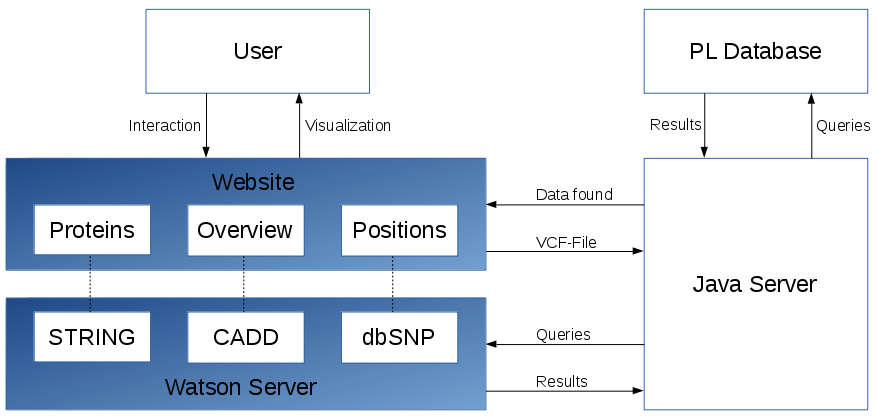
\includegraphics[scale=0.5]{schema1-improvedv2.png}
		\begin{itemize}
			\item Watson server
				\subitem The Watson server owned by the TU Delft hosts the databases STRING\cite{franceschini2013string}, dbSNP\cite{sherry2001dbsnp} and CADD\cite{kircher2014general} and processes queries given by the Java server and returns the results.
			\item Java server
				\subitem The java server makes queries and sends these to Watson. It makes these based on the VCF-file given by the web page. It processes these and determines which data is to be retrieved. The data retrieved is then sent to the web page.
			\item PL database
				\subitem The Programming Life database contains the user and patient information. It is needed to log in and add or view patients.
			\item Website
				\subitem The website receives the VCF-file from the user and passes it on to the JAVA server. When it receives data back from the server it visualizes this for the user.
			\item The user 
				\subitem The user can interact with the website and pick a VCF-file to send. The web page outputs a visualization and the user can draw conclusions from this.
		\end{itemize}
	\subsection{Hardware/software mapping}
		This system will only be used by one type of person, namely a doctor. This means that only one interface will have to be developed and used. A user needs to log on to a web page, after which he or she will be shown a page where VCF-files can be uploaded and analyzed. The web page can be accessed from devices connected to the Internet but is targeted at desktops.
	\subsection{Database Connectivity}
		\begin{itemize}
			\item dbSNP
				\subitem The database dbSNP is used by the java server to get information on the SNP's found in the VCF-file supplied by the user. What is most often retrieved is the gene associated with this SNP so we can use it to search for information about this gene in the STRING database.
			\item STRING
				\subitem The STRING database contains information about genes and proteins and how these are connected. Using information retrieved from dbSNP, we can look at which SNP affects which gene(s) and what genes it/they affect.
			\item CADD
				\subitem The CADD database contains information on how damaging the mutation is. This can be used to determine whether a mutation is harmful or not, and so the doctor can see it might be the cause of a disease.
			\item Programming Life
				\subitem We use an extra database hosted at the webserver to store extra information for the web-application. \\
				The credentials of the users, the doctors, are stored in the database, the passwords are hashed and salted.\\
				Each user can have multiple patients which are linked through the id of the user.
				Some basic information is stored per user including the uploaded VCF-file.
				For every patient the mutations found in the VCF-file are stored as a single mutation, which is linked to each patient with the patients id.\\
				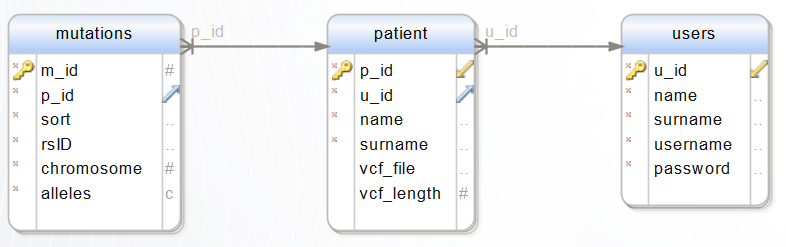
\includegraphics[scale=0.55]{erd.png}
		\end{itemize}
	\subsection{Concurrency }
		At the moment we have no indication how computationally intense our calculations are, thus we cannot say for sure whether or not we will use multiple threads. Until we know more, our program will run on a single thread.
		
